
\subsection{Elección de pares similares}
\subsubsection{Hipótesis}
La siguiente predicción implica que hay una preferencia por interactuar con personas similares o invertir en grupos con personas similares. Esta predicción no se deriva de modelo por el supuesto de que solo el jugador 1 tiene identidad y elige sus expresiones de género, mientras que el jugador 2 solo decide si interactúa o no. Sin embargo, la preferencia por pares similares ha sido identificada como un factor relevante al momento decidir con quién interactuar o con quién ser más prosocial \citep{chakravarty2017discriminationexclusion, halevy2012ingroupoutgroup, chen2009groupidentity, tajfel1971intergroupbehaviour}.

\begin{hyp}
La disposición a interactuar depende de qué tan similares son la persona que elige y la que es elegida. 
\end{hyp}

\subsubsection{Estrategia empírica}
    Para estimar cómo cambia la disposición a interactuar con una persona que es más similar en sus expresiones de género, primero se creó un indicador de si la persona que organizó los perfiles y la persona a la que le asignó un lugar en la lista tenían la misma aspiración y otro de si tenían la misma habilidad. La similitud en la vestimenta de la persona que organizaba los perfiles y la de los perfiles que observaba, está definida por un puntaje entre cero y uno, a partir de la siguiente métrica: 
\begin{equation*}
    similitud\_vestimenta=\frac{1}{1-|puntaje\_vestimenta_i - puntaje\_vestimenta_j|}
\end{equation*}
El puntaje de similitud de vestimenta es creciente en la similitud. Es decir, toma entonces el valor de uno si las dos personas eligieron la misma vestimenta y un valor cercano a cero si uno eligió la vestimenta más femenina y otro eligió la más masculina.

Sea $Ranking_{ij}$ el orden que la persona $i$ le asigna a la persona $j$, $similitud\_vestimenta_{ij}$ el puntaje de similitud entre la vestimenta que eligió la persona $j$ y la persona $i$, $misma\_habilidad_{ij}$ un indicador que toma el valor de uno si la persona $j$ y la persona $i$ reportaron la misma habilidad, $misma\_aspiracion_{ij}$ un indicador que toma el valor de uno si la persona $j$ y la persona $i$ reportaron la misma aspiración, $bogota_j$ un indicador de si la persona $j$ nació en Bogotá, $posicion\_inical_j$ el puesto que tenía la persona $j$ en la lista de la persona $i$ antes de que la persona $i$ reorganizara los perfiles según su preferencia y sea $\gamma_i$ el efecto fijo de la persona $i$; el modelo de esta sección es:
\small{
\begin{equation}
    \begin{split}
	Ranking_{ij}=& \beta_1similitud\_vestimenta_{ij} + \beta_2misma\_habilidad_{ij} \\
	            +& \beta_3misma\_habilidad_{ij}\times similitud\_vestimenta_{ij} + \beta_4misma\_aspiracion_{ij} \\
	            +& \beta_5edad_j +\beta_6bogota_j + \beta_7posicion_inicial_j + \gamma_i + \epsilon_{ij}
    \end{split}
\end{equation}}
A partir de esta ecuación, estimada por MCO, fueron estimadas las pruebas de hipótesis para comprobar si existe una preferencia por desarrollar la tarea con pares similares o no (Hipótesis 4). Las pruebas de hipótesis buscan demostrar si existe diferencia entre el ranking esperado de una persona muy similar (diferente) en sus expresiones de género y el ranking esperado con todas las demás combinaciones de similitud en expresiones de género. Por ejemplo, una de esas pruebas de hipótesis es si existe diferencia en el ranking esperado de una persona que tiene la misma vestimenta, la misma habilidad y la misma aspiración que la persona que ordena la lista y e ranking esperado de una persona con la misma habilidad y aspiración pero con una vestimenta muy diferente. En estas pruebas de hipótesis, una vestimenta muy similar es aquella con un puntaje de similitud de uno, y una vestimenta muy diferente es la que tiene un puntaje de similitud de cero. 

\subsubsection{Resultados}
\begin{table}
    \centering
    \caption{Elección de pares similares}
    \label{tab:my_label}
    \begin{threeparttable} \fontsize{9.5}{12}\selectfont {
    \begin{tabular}{lc} \hline
                                                &   (1)     \\ \hline
                                                &           \\
    Similitud en vestimenta                     &   -1.033* \\
                                                &   (0.574) \\
    Mismas habilidad                            &   -0.588  \\
                                                &   (0.519) \\
    Mismas habilidad*Similitud en vestimenta    &   1.381*  \\
                                                &   (0.829) \\
    Misma aspiración                            &  -0.508** \\
                                                &   (0.215) \\
    Edad                                        &   0.014   \\
                                                &   (0.062) \\
    Bogotá                                      &   -0.111  \\
                                                &   (0.220) \\
    Posición inicial                            &  0.256*** \\
                                                &   (0.045) \\
    Constante                                   &  3.835*** \\
                                                &   (1.341) \\
                                                &           \\
    Observaciones                               &   560     \\
    Número de rankers                           &   70      \\ \hline
    \end{tabular}}
    \begin{tablenotes}
    \scriptsize{
    \item Nota: *** p$<$0.01, ** p$<$0.05, * p$<$0.1; errores estándar robustos en paréntesis.}
    \end{tablenotes}
    \end{threeparttable}
\end{table}

Preferencia por pares muy diferentes o muy similares por encima de pares que son similares en una expresión de género y diferentes en la otra. Sobretodo hay un rechazo a trabajar con personas que tengas una vestimenta muy similar pero diferente habilidad. 

\begin{figure}[htbp]
    \centering
    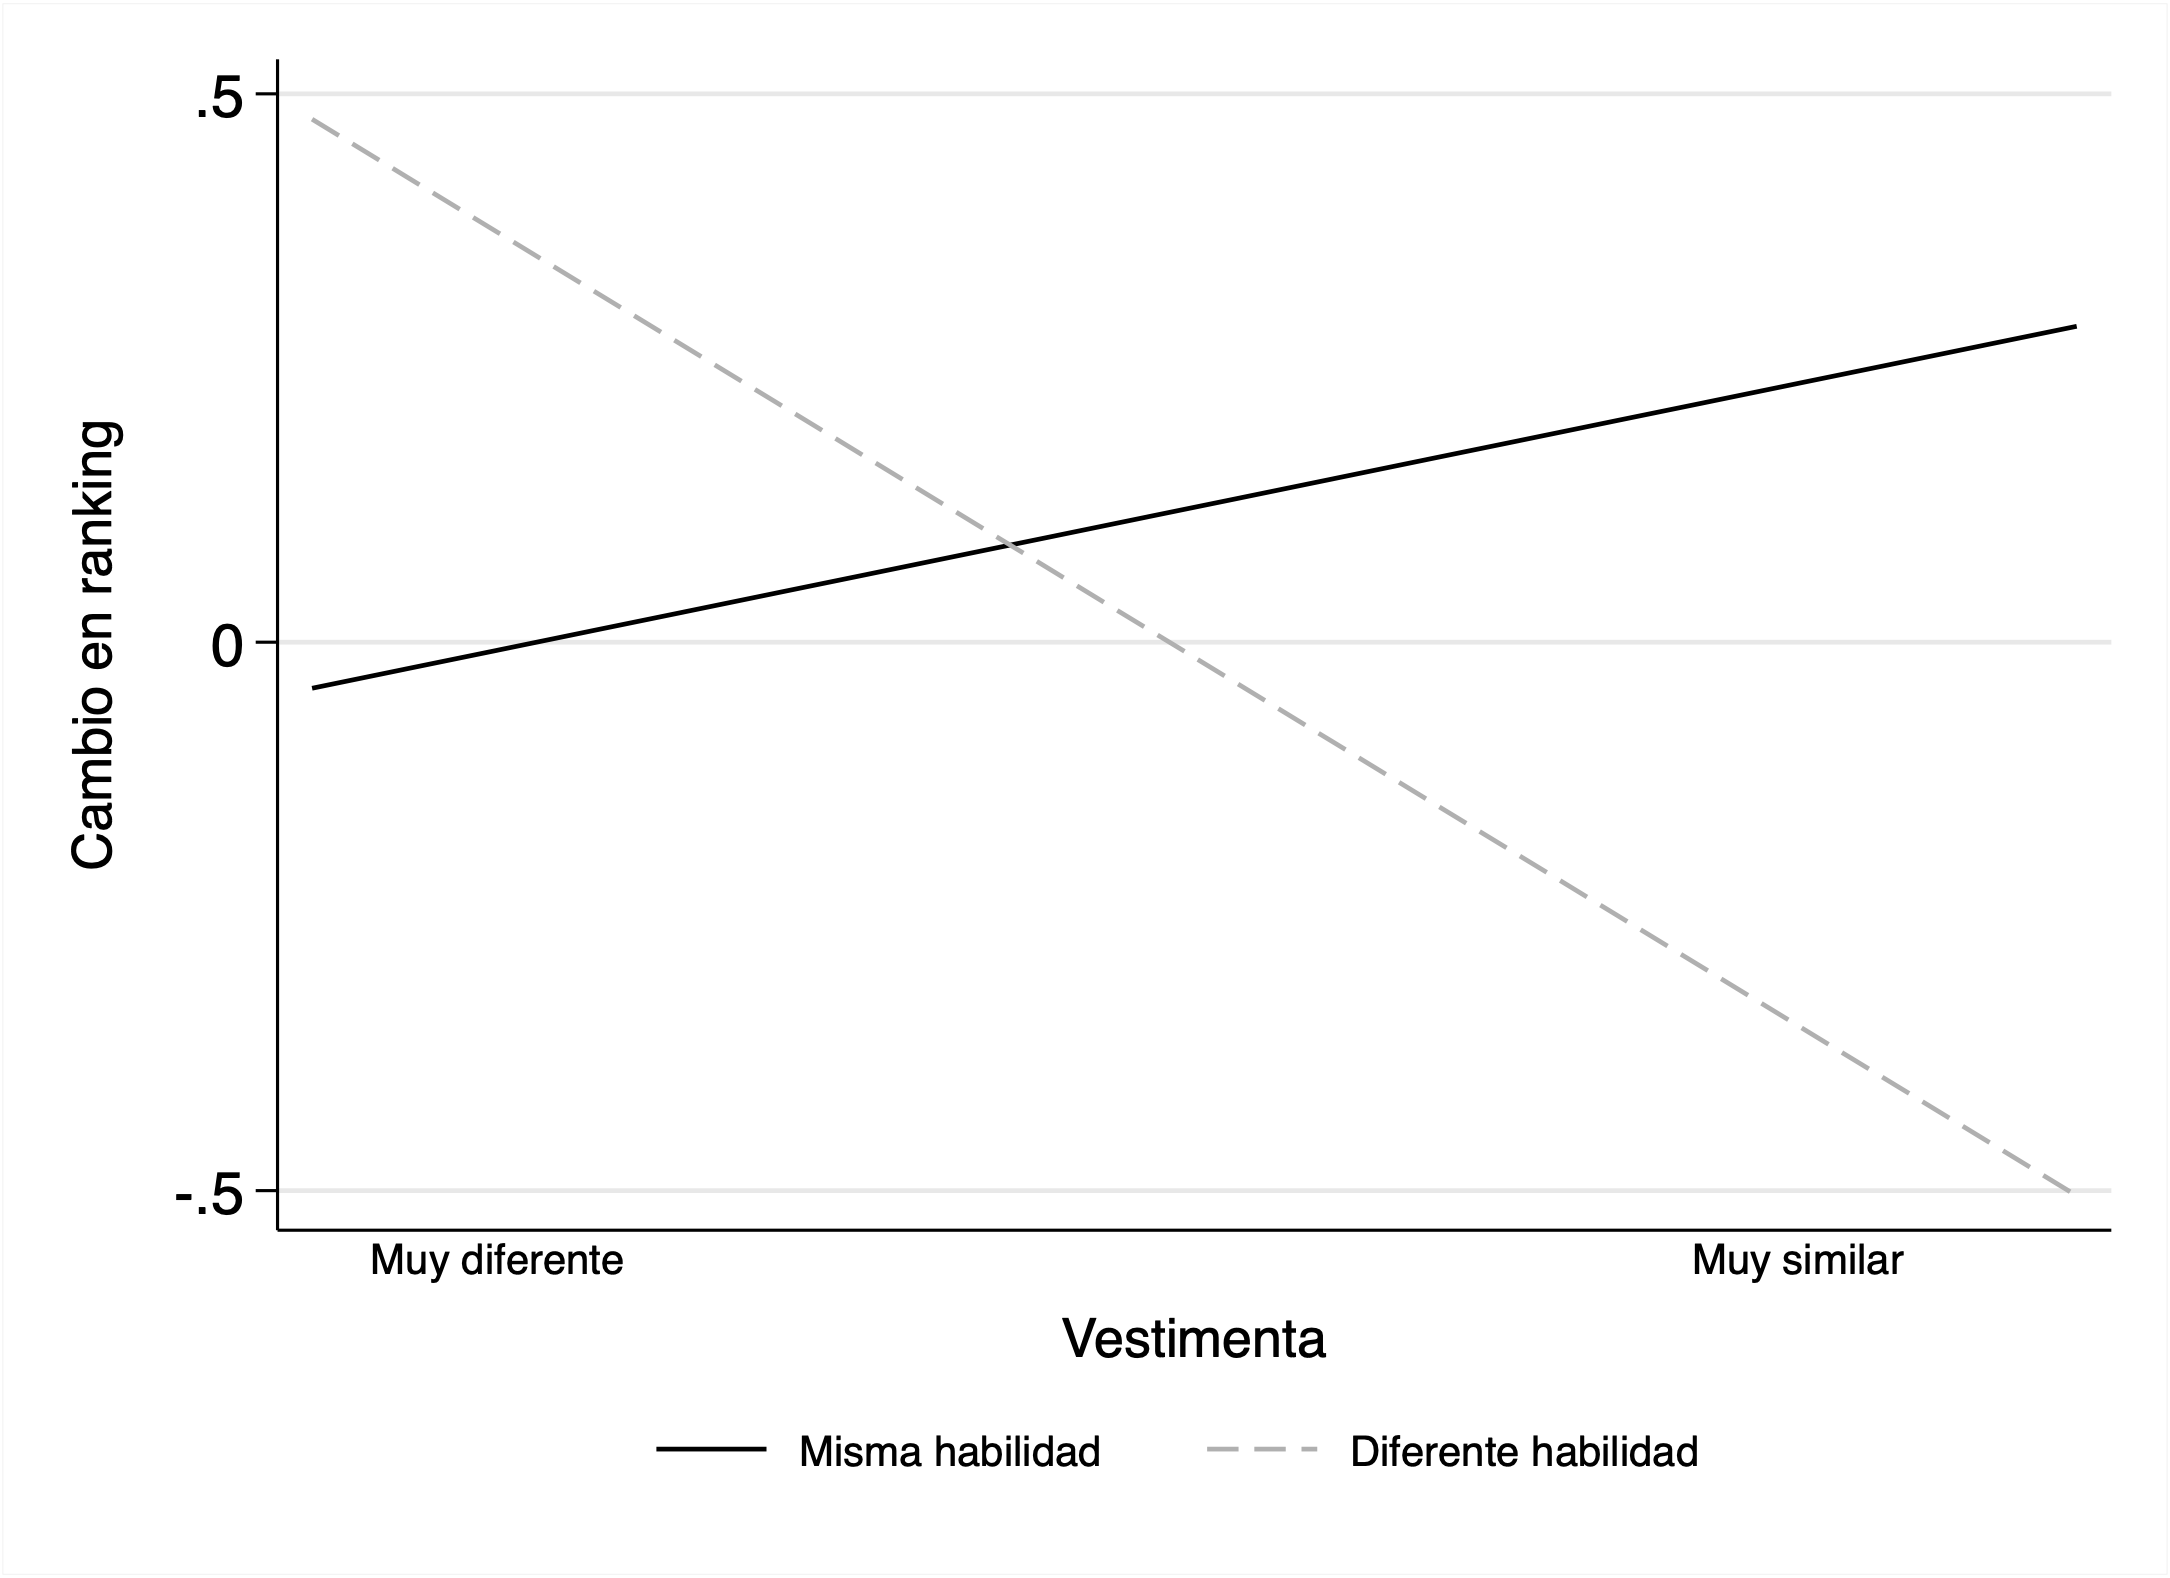
\includegraphics[width=10cm]{Images/h3_predicted_rank_score.png}
    \caption{Ranking esperado por combinaciones de similitud}
    \label{fig:H4}
\end{figure}

\begin{table}
    \centering
    \caption{Diferencia en ranking por similitud en expresiones de género}
    \label{tab:H4}
    \begin{threeparttable} \fontsize{9.5}{12}\selectfont {
    \begin{tabular}{|cc|cccc|}\hline
    
            	&	\textbf{V}	&	M	&	M	&	D	&	D	\\
    \textbf{V}	&	\textbf{H}	&	M	&	D	&	M	&	D	\\ \hline
    M	        &	M	        &   -	& 0.79* &  0.35	& -0.24	\\
    D	        &	D	        & 0.24	& 1.03*	&  0.59	&   -   \\ \hline

    \end{tabular}}
    \begin{tablenotes}
    \scriptsize{
    \item Nota: V corresponde a la vestimenta, A a la aspiración y H a la habilidad. M corresponde a misma expresión y D a diferente expresión de género, es decir si tienen la misma aspiración en la fila/columna A aparece M y si tienen una aspiración diferente aparece D. Los valores de la tabla corresponden a la fila menos la columna. Si el valor es positivo, es porque la combinación de expresiones de género de la fila tiene un mejor ranking que la combinación de la columna. Por ejemplo una persona con todas sus expresiones iguales de quien organiza los perfiles, en promedio está 0.81 puestos arriba de una persona que tiene la misma vestimenta, la misma aspiración, pero diferente habilidad (la fila superior en la segunda columna).}
    \end{tablenotes}
    \end{threeparttable}
\end{table}


\begin{result}
La disposición a interactuar no depende de qué tan similares son la persona que elige y la que es elegida. 
\end{result}


